

% A Readymade beamer presentation template
% Version 1.1
% Relase date: May 2, 2010
% Released at http://www.stattler.com
% by Rifat Jahan

\documentclass{beamer}
%\usecolortheme[named=green]{structure}
\mode<presentation> {
\usetheme{CambridgeUS}
\usecolortheme{orchid}
\usefonttheme{structuresmallcapsserif}
%\setbeamercovered{invisible}
% To remove the navigation symbols from the bottom of slides%
\setbeamertemplate{navigation symbols}{} 
}
 \setbeamertemplate{footline}
        {
      \leavevmode
      \hbox{
      \begin{beamercolorbox}[wd=.36\paperwidth,ht=2.25ex,dp=1ex,center]{author in head/foot}
        \usebeamerfont{author in head/foot}\insertshortauthor~~(\insertshortinstitute)
      \end{beamercolorbox}
      \begin{beamercolorbox}[wd=.56\paperwidth,ht=2.25ex,dp=1ex,center]{title in head/foot}
        \usebeamerfont{title in head/foot}\insertshorttitle
      \end{beamercolorbox}
      \begin{beamercolorbox}[wd=.08\paperwidth,ht=2.25ex,dp=1ex,right]{date in head/foot}
        \usebeamerfont{date in head/foot}\insertframenumber{}\hspace*{2em}

      \end{beamercolorbox}}
      \vskip0pt
    }

\usepackage{graphicx}
\title[Excepted Appointments and Presidential Unilateral Power]{Excepted Appointments and Presidential Unilateral Power}
%
\author{Emily Moore}
\institute[WUSTL]
{
Washington University-St. Louis \\
\medskip
{\emph{emily.moore@wustl.edu}}
}
\date{April 22, 2016}
% \today will show current date. 
% Alternatively, you can specify a date.

\usepackage{Sweave}
\begin{document}
\Sconcordance{concordance:MooreWISEPresentationSlides.tex:MooreWISEPresentationSlides.Rnw:%
1 49 1 1 0 202 1}


%
\begin{frame}
\titlepage
\end{frame}
%
%

\begin{frame}
\frametitle{Presidents Influencing Policy}
\large
\begin{itemize}\addtolength{\itemsep}{.75\baselineskip}
\item Presidents need ways to both pursue their agendas and keep the government running without relying exclusively on Congress.
\item Presidents have many tools for influencing legislative and administrative policymaking.
\item Appointment power is one of these tools (e.g., Moe 1985; Lewis 2008).
\item Scholars and journalists have increasingly turned their attention to unilateral powers, but excepted appointments have gone largely unrecognized as one of these powers. 
\end{itemize}
\hfill%
\end{frame}

%\begin{frame}
%\frametitle{Contribution}
%\large
%\centering
%Though some limited work has been produced on excepted appointees, no studies to date have examined the use of these appointees during periods of ideological conflict within the Senate. I argue that excepted appointees are a consequential political tool that the president will utilize in greater numbers when conditions within the Senate make pursuing policies more difficult.
%\hfill%
%\end{frame}


\begin{frame}
\frametitle{Warren and Weiss}
\begin{center}
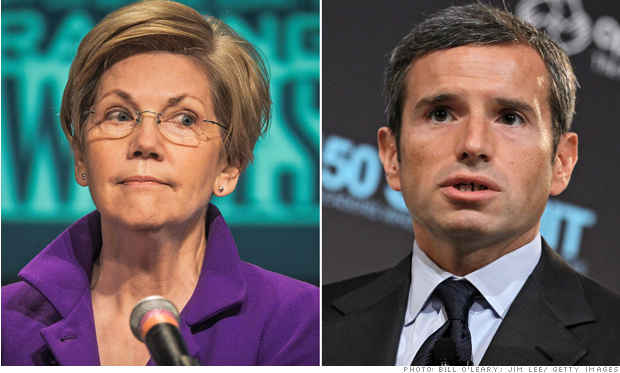
\includegraphics[height=2.6in,width=4in]{WarrenWeiss.png}

Elizabeth Warren and Antonio Weiss
\end{center}
\end{frame}

\begin{frame}
\frametitle{Lessons from the Warren and Weiss Story}
\large
Excepted appointments allow the president to...
\bigskip
\begin{itemize}\addtolength{\itemsep}{0.5\baselineskip}
\item avoid the lengthy confirmation process and the embarrassment of unconfirmed nominees.
\item staff agencies quickly.
\item staff agencies when Congress is unable to come to a consensus about a nominee.
\item utilize talented potential nominees who cannot go through the confirmation process. 
\end{itemize}
\end{frame}

\begin{frame}
\frametitle{Why Do Presidents Need Excepted Appointees?}
\large
\begin{itemize}\addtolength{\itemsep}{0.25\baselineskip}
\item The length of time to confirmation has increased substantially since the 1980s. Appointees wait an average of nine months for confirmation.
\item Over 25 percent of nominees are never confirmed.
\item Top positions in agencies are vacant or filled by acting officials 15-25 percent of the time.
\item Long wait times discourage talented people from working in the government.
\end{itemize}
\end{frame}

\begin{frame}
\frametitle{Theory 1}
\large
\begin{itemize}\addtolength{\itemsep}{1\baselineskip}
\item Consistent with other literature on unilateral powers, presidents would prefer to work with Congress as much as possible, but when Congress is gridlocked, presidents are willing to act alone.
\item \textit{H1: When ideological conflict within the Senate is high, presidents will utilize Schedule C appointees more frequently.}  
\end{itemize}
\end{frame}

\begin{frame}
\frametitle{The Case of Schedule C}
\large
Schedule C appointees...
\begin{itemize}\addtolength{\itemsep}{0.75\baselineskip}
\item are a unique type of excepted appointment created by Eisenhower.
\item serve in special positions created just for them.
\item serve in ``confidential or policy-determining" positions.
\end{itemize}
\bigskip
\bigskip
Like all excepted appointees, they do not undergo advice and consent nor are they subject to competitive hiring processes. 
\end{frame}

\begin{frame}
\frametitle{Examples of Schedule Cs in the larger system}
\begin{itemize}\addtolength{\itemsep}{1.5\baselineskip}
\item PAS appointees serve as department secretaries and undersecretaries as well as heads of independent agencies.
\item Deputy Undersecretaries are often non-career SES. 
\item Schedule Cs have many different jobs, but often serve as advisors on specific policy matters and sometimes approve the rulemaking activities of career staff or serve as liaison between political and career appointees.
\end{itemize}
\hfill%
\end{frame}


\begin{frame}
\frametitle{Data}
\begin{itemize} \addtolength{\itemsep}{1.5\baselineskip}
\item Data come from OPM, including all appointees who do not undergo advice and consent from 1998-2013.
\item Few studies utilize these data.
\item 692 agencies exist over the period with varying levels of agency aggregation. 
\item Within the agency, we can determine total employment broken down by appointment type. 
\end{itemize}
\end{frame}

\begin{frame}
\frametitle{Total Schedule Cs and New Hires Over Time}
\centering
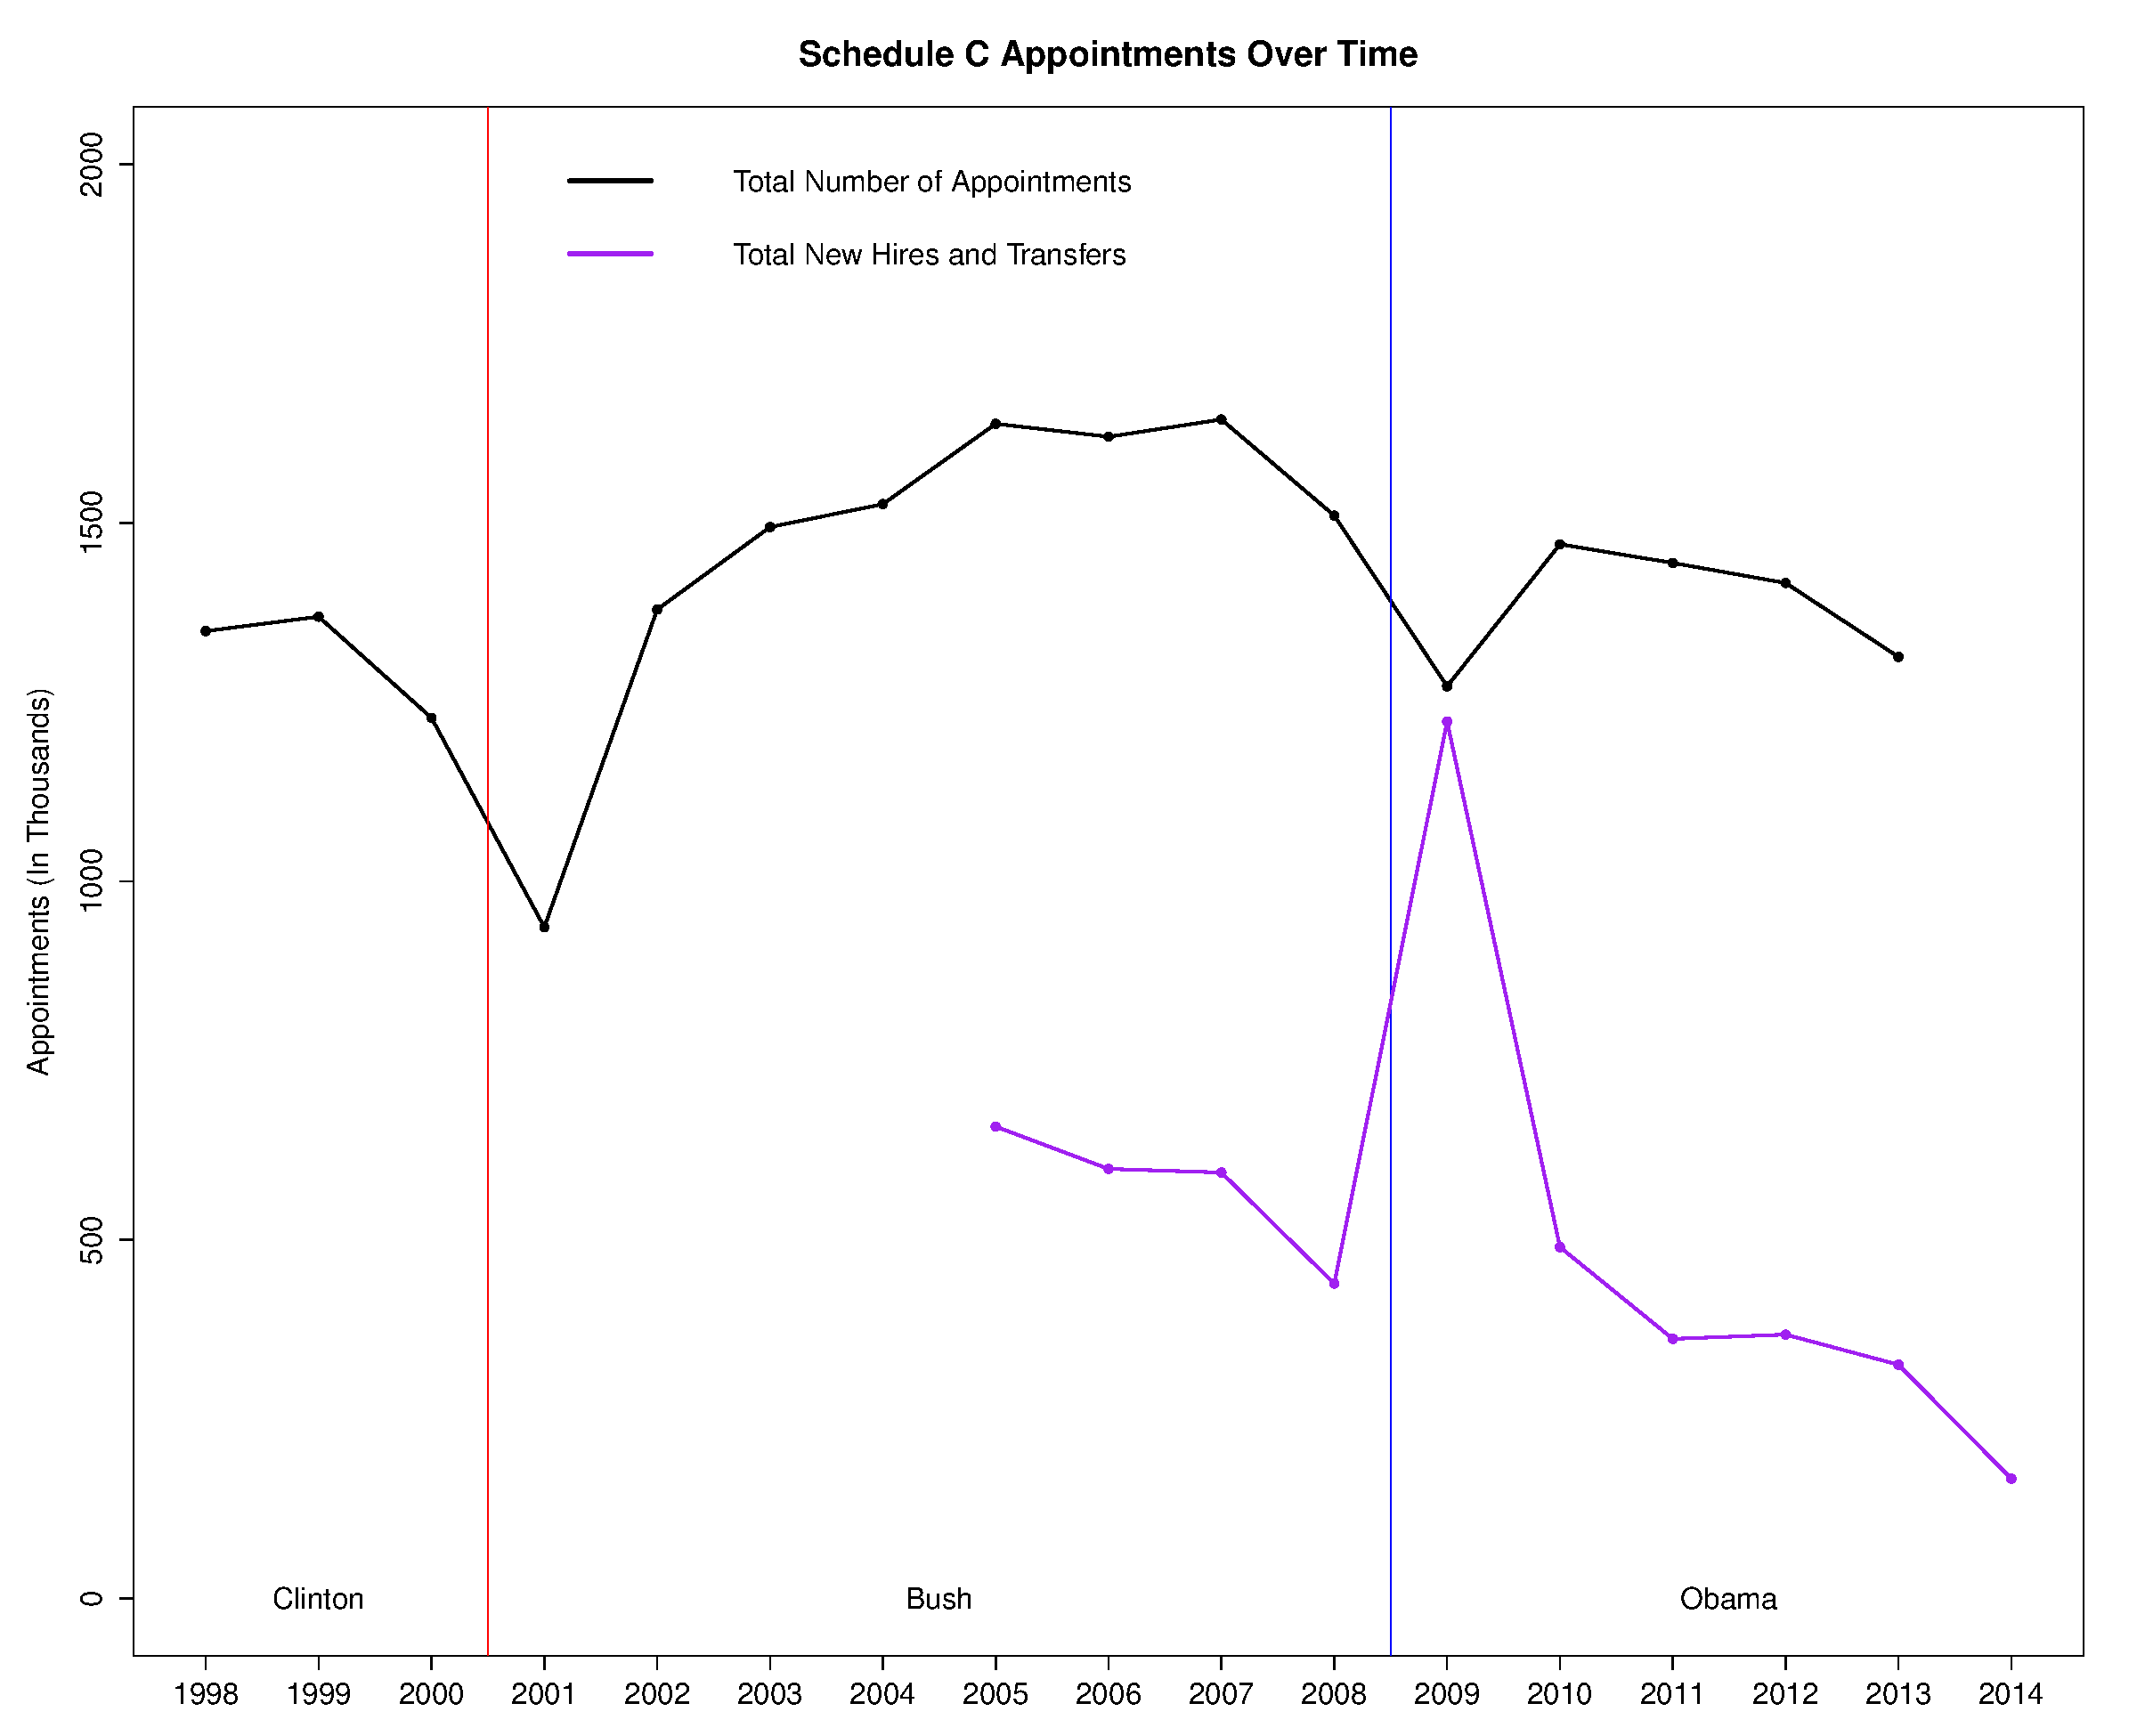
\includegraphics[height=3.1in,width=4in]{SCAptsandAccOverTime.pdf}
\end{frame}

\begin{frame}
\frametitle{Method}
\begin{itemize}\addtolength{\itemsep}{0.25\baselineskip}
\item Negative Binomial regression model with clustered standard errors.
\item \textbf{Dependent variable:} number of Schedule C appointees in an agency each year, 1998-2013.
\item \textbf{Intra-branch conflict in the Senate:} Ideological Distance between party medians.
\item Controls include agency ideology (Chen and Johnson scores), distance president to 60th senator, agency size (total appointments), first and last year of presidency and president dummies. 
\end{itemize}
\end{frame}

%\begin{frame}
%\frametitle{2013 Agency Counts of Schedule C Appointees}
%\scriptsize
%\begin{table}[ht]
%\centering
%\begin{tabular}{lc}
%  \hline
%\textbf{Top 10 Agencies} & Number of Schedule Cs in 2013 \\
%\hline
%Department of Agriculture & 150\\ 
%Department of Education & 111 \\ 
%Department of State & 88 \\ 
%Department of Defense & 83  \\ 
%Department of Commerce & 75 \\ 
%Department of Labor & 74\\ 
%Department of Health and Human Service & 69\\ 
%Department of Energy & 68 \\ 
%Department of Homeland Security & 62  \\ 
%Department of Justice & 57\\ 
%\hline
%\textbf{Bottom 10 Agencies} & Number of Schedule Cs in 2013 \\
%\hline
%National Science Foundation & 0\\ 
%National Council on Disability & 0 \\ 
%National Labor Relations Board & 0 \\ 
%National Archives and Records Administration & 0 \\ 
%Nuclear Regulatory Commission& 0 \\ 
%Peace Corps & 0\\ 
%Railroad Retirement Board& 0 \\ 
%Smithsonian Institute & 0\\ 
%National Transportation Safety Board& 0 \\ 
%Trade Deficit Review Commission& 0\\ 
%   \hline
%\end{tabular}
%\end{table}
%\end{frame}

\begin{frame}
\frametitle{Results}
\centering
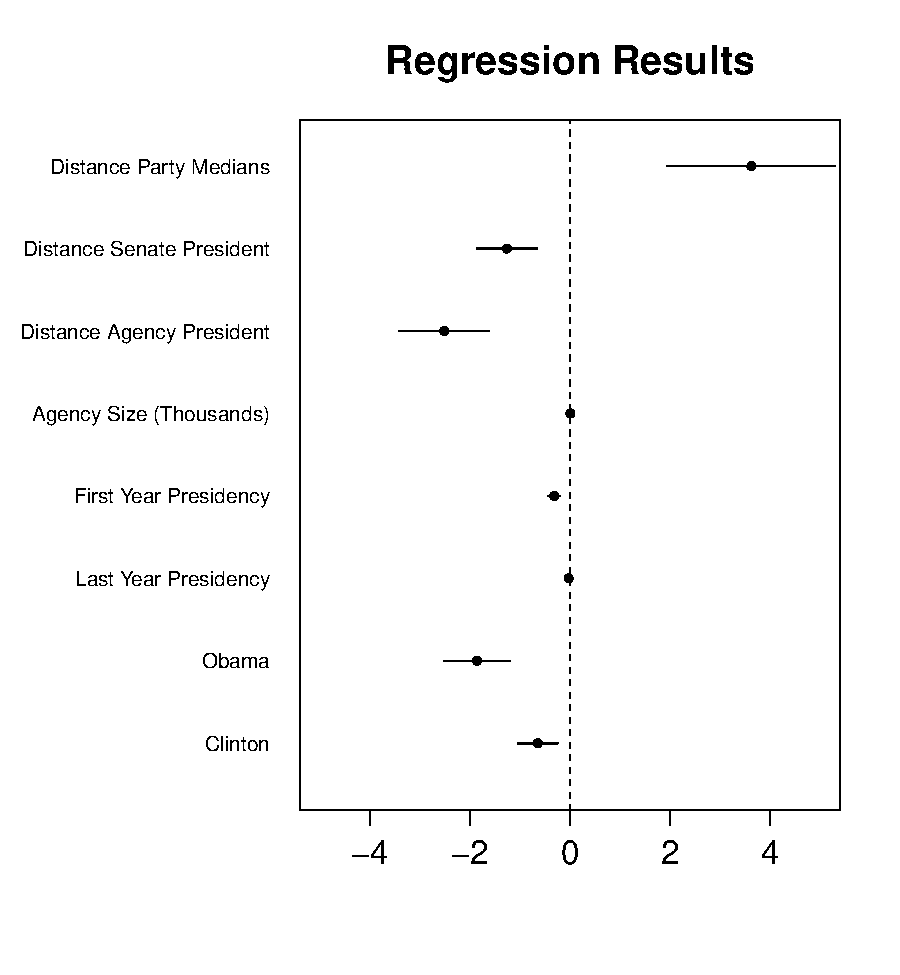
\includegraphics[height=3.4in,width=3.2in]{CoefficientPlot.pdf}
\end{frame}

\begin{frame}
\frametitle{Results Plot}
\centering
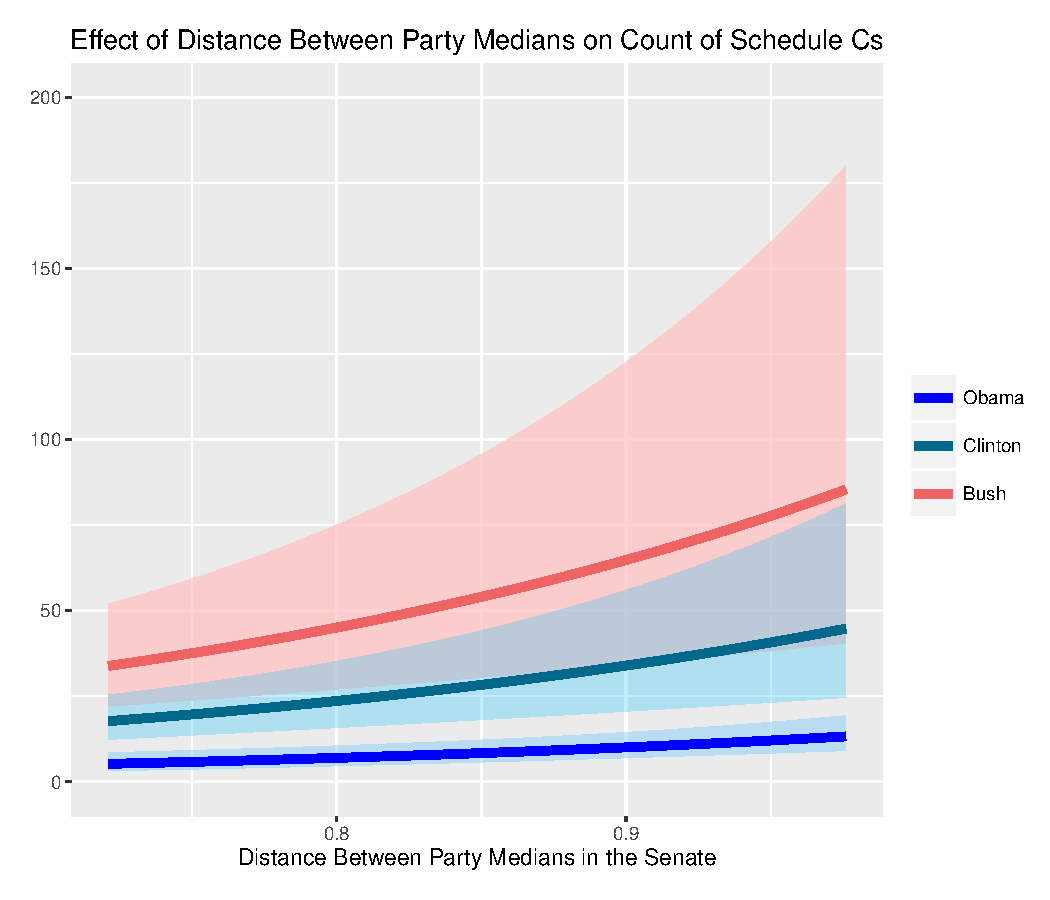
\includegraphics[height=3.1in,width=3.5in]{ResultsPlots.pdf}
\end{frame}

\begin{frame}
\frametitle{Conclusion}
\large
\begin{itemize}\addtolength{\itemsep}{0.75\baselineskip}
\item Excepted Appointees---and especially Schedule C appointees---are a consequential but understudied unilateral policy tool.
\item With the increasing length of time to confirmation and increasing polarization in Congress, presidents need the flexibility excepted appointments provide.
\item Because presidents need to continue to pursue their agendas and keep the government running when the Senate faces internal conflict, presidents will utilize Schedule C appointees more frequently when conflict within the Senate is high. 
\end{itemize}
\end{frame}

\begin{frame}
\frametitle{Further Research}
\large
\begin{itemize}\addtolength{\itemsep}{1.75\baselineskip}
\item Looking at how leadership vacancies in agencies affect Schedule C appointees is a natural extension.
\item In addition, little is known about how appointees---both Schedule C and other appointment types---are related to regulatory output.
\item This rulemaking dataset also includes a number of interesting variables itself, including each rule's citation to authority in the U.S. Code, CFR, and executive orders. 
\end{itemize}
\end{frame}

\end{document}









